\documentclass[11pt]{article}
\usepackage[margin=1in]{geometry}
\usepackage{hyperref}
\usepackage{booktabs}
\usepackage{graphicx}
\usepackage{enumitem}
\setlist{nosep}

\title{A Small Work-Stealing Task Runtime: Milestone}
\author{Roger Yang (hryang)}
\date{15-418, November 23, 2026}

\begin{document}
\maketitle

\noindent\textbf{URL:} \url{https://rogeryang85.github.io/work-stealing-runtime/}

\section*{Focus}
Per the proposal feedback, I'm not trying to beat Cilk or OpenMP. The focus is how
the runtime scales and how much each design choice matters. It's a plain C++
library with no compiler support, so programs must be strict fork-join
(\texttt{spawn}/\texttt{wait} in a \texttt{TaskGroup}), and thieves steal children
instead of continuations.

\section*{Progress}
Done: a Chase--Lev deque per thread with random stealing, a central-queue
scheduler with the same API, and fib, quicksort, n-queens and UTS in serial, my
runtime and OpenMP. All results are checked against serial. This matches the
proposal schedule.

\section*{Preliminary results}
M3 Pro laptop, 6 performance cores, median of 5 runs. GHC runs are next.

\begin{center}
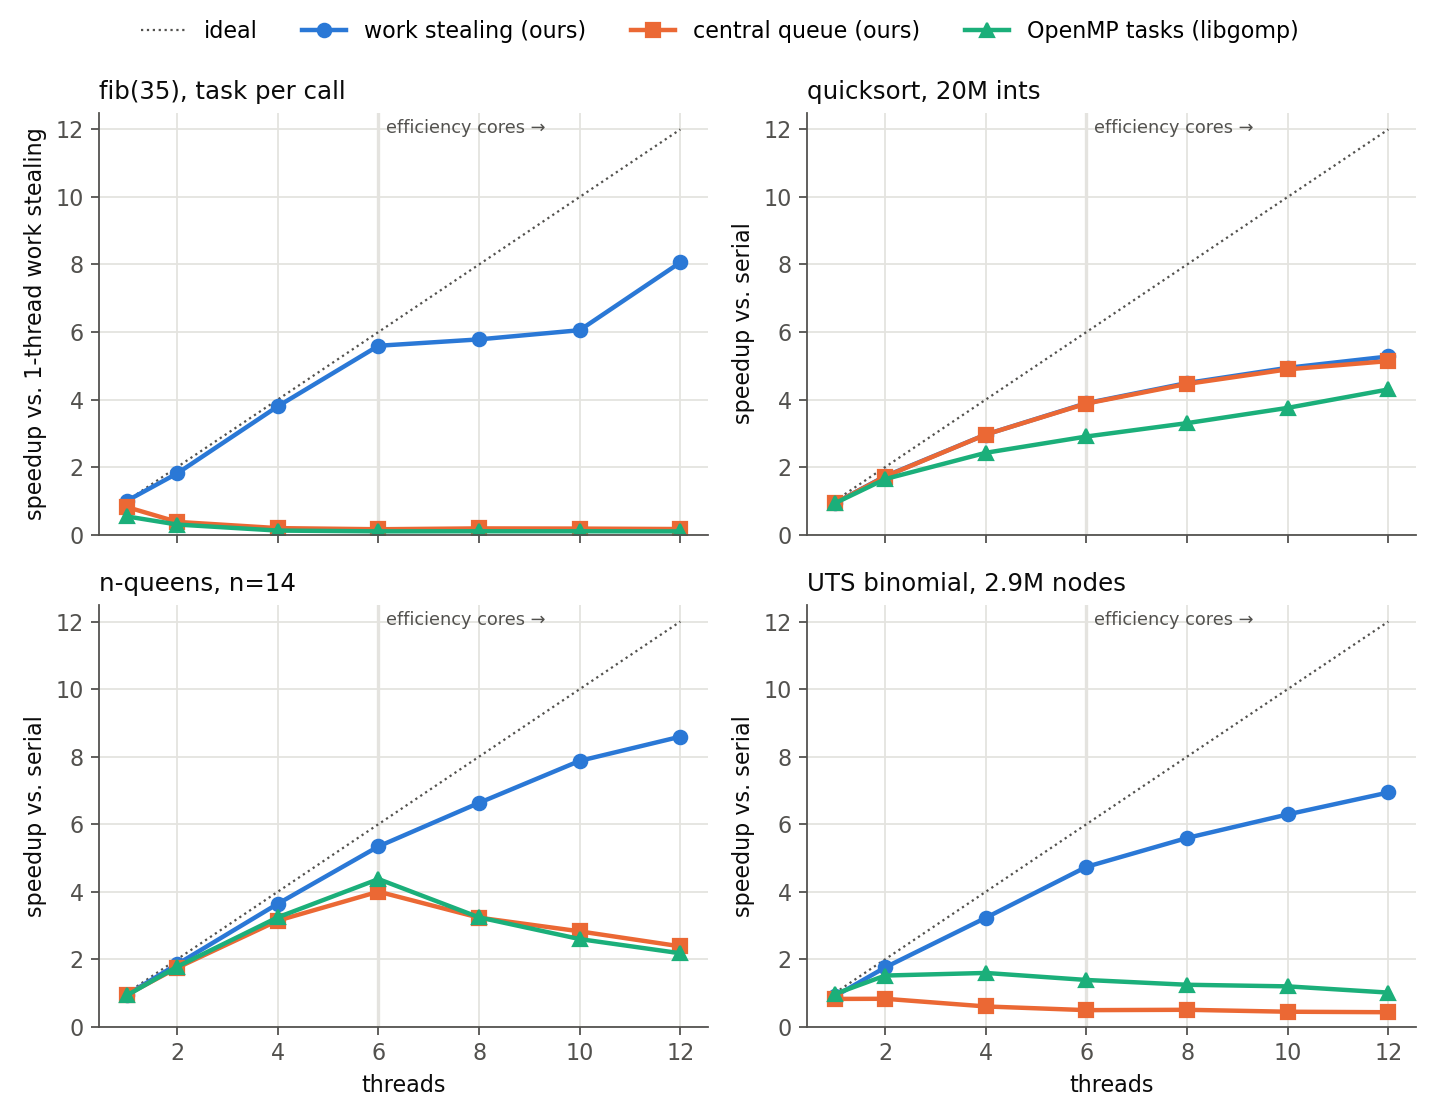
\includegraphics[width=0.62\textwidth]{mac_speedup.png}

\medskip
\begin{tabular}{@{}lrrr@{}}
\toprule
Speedup at 6 threads & work stealing & central queue & libgomp (ref.) \\
\midrule
fib(35)$^*$     & 5.3$\times$ & 0.22$\times$ & 0.15$\times$ \\
quicksort, 20M  & 3.4$\times$ & 3.7$\times$  & 2.8$\times$ \\
n-queens, n=14  & 5.3$\times$ & 3.6$\times$  & 4.3$\times$ \\
UTS, 2.9M nodes & 4.6$\times$ & 0.38$\times$ & 1.3$\times$ \\
\bottomrule
\end{tabular}\\[2pt]
{\small $^*$vs.\ my runtime on 1 thread, with one task per call. The rest are vs.\ serial.}
\end{center}

\noindent With tiny tasks, the central queue gets slower as threads are added, while
per-thread deques keep scaling. Each task costs about 27\,ns. Quicksort is limited
by its serial first partition.

\section*{Remaining goals}
Each one is a design choice, measured on GHC (8 cores):
\begin{itemize}
  \item task allocation: \texttt{new}/\texttt{delete} vs.\ per-thread pools
  \item victim choice: random vs.\ round-robin vs.\ last successful victim
  \item idle threads: spin vs.\ yield vs.\ sleep
  \item task granularity (cutoff sweeps)
\end{itemize}
Stretch: lazy binary splitting. The poster will show scaling graphs for each choice
plus a per-thread UTS timeline. No live demo.

\section*{Concerns}
None blocking. Some runs are only 10--20\,ms, so I'll use bigger inputs on GHC.

\section*{Schedule}
All tasks are mine (Roger).

\medskip
\begin{tabular}{@{}ll@{}}
\toprule
Nov 23--25    & GHC runs, deque test on x86, bigger inputs \\
Nov 26--29    & Thanksgiving; task pools \\
Nov 30--Dec 2 & Steal policies \\
Dec 3--6      & Idle policies, granularity, UTS timeline \\
Dec 7--8      & Final GHC runs; lazy binary splitting if ahead \\
Dec 9--10     & Final report \\
Dec 11        & Poster session \\
\bottomrule
\end{tabular}

\end{document}
